\chapter{Simulation methods}\label{chap5}

In the previous chapters, we focused on conjugate families, where the posterior and predictive distributions have standard analytical forms (e.g., normal, Student's t, gamma, binomial, Poisson, etc.) and where the marginal likelihood has a closed-form analytical solution. However, realistic models are often more complex and lack such closed-form solutions.

To address this complexity, we rely on simulation (stochastic) methods to draw samples from posterior and predictive distributions. This chapter introduces posterior simulation, a cornerstone of Bayesian inference. We discuss Markov Chain Monte Carlo (MCMC) methods, including Gibbs sampling, Metropolis-Hastings, and Hamiltonian Monte Carlo, as well as other techniques like importance sampling and sequential Monte Carlo.

The simulation methods discussed in this chapter are specifically applied throughout this book. However, we do not delve into deterministic methods, such as numerical integration (quadrature), or other simulation methods, including discrete approximation, the probability integral transform, the method of composition, accept-reject sampling, and slice sampling algorithms. While these methods are also widely used, they are not as common as the approaches explicitly employed in this book.

For readers interested in these alternative methods, we recommend exploring \cite[Chaps.~2 and 3]{robert2010introducing}, \cite[Chaps.~2, 3, and 8]{robert2011monte}, \cite[Chap.~5]{greenberg2012introduction}, and \cite[Chap.~10]{gelman2021bayesian}.

\section{Markov chain Monte Carlo methods}\label{sec51}

Markov Chain Monte Carlo (MCMC) methods are algorithms used to approximate complex probability distributions by constructing a Markov chain. This chain is a sequence of random samples where each sample depends only on the previous one. The goal of MCMC methods is to obtain draws from the posterior distribution as the equilibrium distribution. The key point in MCMC methods is the transition kernel or density, $q(\bm{\theta}^{(s)}|\bm{\theta}^{(s-1)})$, which generates a draw $\bm{\theta}^{(s)}$ at stage $s$ that depends solely on $\bm{\theta}^{(s-1)}$. This transition distribution must be designed such that the Markov chain converges to a unique stationary distribution, which, in our case, is the posterior distribution, that is, $\pi(\bm{\theta}^{(s)}|\bm{y})=\int_{\bm{\Theta}}q(\bm{\theta}^{(s)}|\bm{\theta}^{(s-1)})\pi(\bm{\theta}^{(s-1)}|\bm{y})d\bm{\theta}^{(s-1)}$.

Given that we start at an arbitrary point, $\bm{\theta}^{(0)}$, the algorithm requires that the Markov chain be \textit{irreducible}, meaning that the process can reach any other state with positive probability. Additionally, the process must be \textit{aperiodic}, meaning that for each state, the greatest common divisor of the number of steps it takes to return to the state is 1, ensuring that there are no cycles forcing the system to return to a state only after a fixed number of steps. Furthermore, the process must be \textit{recurrent}, meaning that it will return to any state an infinite number of times with probability one. However, to ensure convergence to the stationary distribution, a stronger condition is required: the process must be \textit{positive recurrent}, meaning that the expected return time to a state is finite. Given an \textit{irreducible}, \textit{aperiodic}, and \textit{positive recurrent} transition density, the Markov chain algorithm will asymptotically converge to the stationary posterior distribution we are seeking. For more details, see \cite[chap.~6]{robert2011monte}.
   

\subsection{Gibbs sampler}\label{sec511}

This Gibbs sampler algorithm is one of the most widely used MCMC methods for sampling from non-standard distributions in Bayesian analysis. While it is a special case of the Metropolis-Hastings (MH) algorithm, it originated from a different theoretical background \cite{Geman1984,Gelfand1990}. The key requirement for implementing the Gibbs sampling algorithm is the availability of conditional posterior distributions. The algorithm works by cycling through the conditional posterior distributions corresponding to different blocks of the parameter space under inference.

Two simplify concepts let's focus on a parameter space composed by two blocks, $\bm{\theta} = [\bm{\theta}_1 \ \bm{\theta}_2]^{\top}$, the Gibbs sampling algorithm uses as transition kernel $q(\bm{\theta}_1^{(s)},\bm{\theta}_2^{(s)}|\bm{\theta}_1^{(s-1)},\bm{\theta}_2^{(s-1)})=\pi(\bm{\theta}_1^{(s)}|\bm{\theta}_2^{(s-1)},\bm{y})\pi(\bm{\theta}_2^{(s)}|\bm{\theta}_1^{(s)},\bm{y})$. Thus,
{\scriptsize
\begin{align*}
	\int_{\bm{\Theta}}q(\bm{\theta}^{(s)}|\bm{\theta}^{(s-1)})\pi(\bm{\theta}^{(s-1)}|\bm{y})d\bm{\theta}^{(s-1)}
	&=\int_{\bm{\Theta}_2}\int_{\bm{\Theta}_1}\pi(\bm{\theta}_1^{(s)}|\bm{\theta}_2^{(s-1)},\bm{y})\pi(\bm{\theta}_2^{(s)}|\bm{\theta}_1^{(s)},\bm{y})\pi(\bm{\theta}^{(s-1)}_1,\bm{\theta}^{(s-1)}_2|\bm{y})d\bm{\theta}^{(s-1)}_1d\bm{\theta}^{(s-1)}_2\\
	&=\pi(\bm{\theta}_2^{(s)}|\bm{\theta}_1^{(s)},\bm{y})\int_{\bm{\Theta}_2}\int_{\bm{\Theta}_1}\pi(\bm{\theta}_1^{(s)}|\bm{\theta}_2^{(s-1)},\bm{y})\pi(\bm{\theta}^{(s-1)}_1,\bm{\theta}^{(s-1)}_2|\bm{y})d\bm{\theta}^{(s-1)}_1d\bm{\theta}^{(s-1)}_2\\
	&=\pi(\bm{\theta}_2^{(s)}|\bm{\theta}_1^{(s)},\bm{y})\int_{\bm{\Theta}_2}\pi(\bm{\theta}_1^{(s)}|\bm{\theta}_2^{(s-1)},\bm{y})\pi(\bm{\theta}^{(s-1)}_2|\bm{y})d\bm{\theta}^{(s-1)}_2\\
	&=\pi(\bm{\theta}_2^{(s)}|\bm{\theta}_1^{(s)},\bm{y})\int_{\bm{\Theta}_2}\pi(\bm{\theta}_1^{(s)},\bm{\theta}_2^{(s-1)}|\bm{y})d\bm{\theta}^{(s-1)}_2\\
	&=\pi(\bm{\theta}_2^{(s)}|\bm{\theta}_1^{(s)},\bm{y})\pi(\bm{\theta}_1^{(s)}|\bm{y})\\
	&=\pi(\bm{\theta}_1^{(s)},\bm{\theta}_2^{(s)}|\bm{y}).\\
\end{align*}
}
Then, $\pi(\bm{\theta}|\bm{y})$ is the stationary distribution for the Gibbs transition kernel.

A word of caution! Even if we have well-defined conditional posterior distributions $\pi(\bm{\theta}_1^{(s)} | \bm{\theta}_2^{(s-1)}, \bm{y})$ and $\pi(\bm{\theta}_2^{(s)} | \bm{\theta}_1^{(s)}, \bm{y})$, and we can simulate from them, the joint posterior distribution $\pi(\bm{\theta}_1^{(s)}, \bm{\theta}_2^{(s)} | \bm{y})$ may not correspond to any proper distribution. We should be mindful of this situation, especially when dealing with improper prior distributions (see \cite[Chap.~10]{robert2011monte} for details).

Algorithm \ref{Alg:Gibbs} shows how to implement a Gibbs sampler with $d$ blocks. 

\begin{algorithm}[h!]
	\caption{Gibbs sampling}\label{Alg:Gibbs}
	\begin{algorithmic}[1]  		 			
		\State Set $\bm{\theta}_2^{(0)}$, $\bm{\theta}_3^{(0)}$, ..., $\bm{\theta}_d^{(0)}$
		\For{\texttt{$s=1,\dots,S$}}
		\State Draw $\bm{\theta}_1^{(s)}$ from $\pi(\bm{\theta}_1^{(s)}|\bm{\theta}_2^{(s-1)},\dots,\bm{\theta}_d^{(s-1)},\bm{y})$
		\State Draw $\bm{\theta}_2^{(s)}$ from $\pi(\bm{\theta}_2^{(s)}|\bm{\theta}_1^{(s)},\dots,\bm{\theta}_d^{(s-1)},\bm{y})$
		\State $\vdots$
		\State Draw $\bm{\theta}_d^{(s)}$ from $\pi(\bm{\theta}_d^{(s)}|\bm{\theta}_1^{(s)},\dots,\bm{\theta}_{d-1}^{(s)},\bm{y})$ 
		\EndFor 
		\end{algorithmic} 
\end{algorithm}

\textbf{Example: Mining disaster change point}

Let's use the dataset \textit{Mining.csv} provided by \cite{carlin1992hierarchical}. This dataset records the number of mining disasters per year from 1851 to 1962 in British coal mines.

We assume there is an unknown structural change point in the number of mining disasters, where the parameters of the Poisson distributions change. In particular,
\begin{align*}
	p(y_t)=\begin{Bmatrix}
		\frac{\exp(-\lambda_1)\lambda_1^{y_t}}{y_t!}, & t=1,2,\dots,H\\
		\frac{\exp(-\lambda_2)\lambda_2^{y_t}}{y_t!}, & t=H+1,\dots,T\\
	\end{Bmatrix},
\end{align*}  
where $H$ is the changing point.

We use conjugate families for $\lambda_l$, $l = 1, 2$, where $\lambda_l \sim G(\alpha_{l0}, \beta_{l0})$, and set $\pi(H) = 1 / T$, which corresponds to a discrete uniform distribution for the change point. This implies that, a priori, we assume equal probability for any time to be the change point.

The posterior distribution is
\begin{align*}
	\pi(\lambda_1,\lambda_2,H|\bm{y})&\propto \prod_{t=1}^{H} \frac{\exp(-\lambda_1)\lambda_1^{y_t}}{y_t!} \prod_{t=H+1}^{T}\frac{\exp(-\lambda_2)\lambda_2^{y_t}}{y_t!}\\
	&\times \exp(-\beta_{10}\lambda_1)\lambda_1^{\alpha_{10}-1} \exp(-\beta_{20}\lambda_2)\lambda_2^{\alpha_{20}-1} 1/T\\
	&\propto\exp(-H\lambda_1)\lambda_1^{\sum_{t=1}^H y_t}\exp(-(T-H)\lambda_2)\lambda_2^{\sum_{t=H+1}^T y_t}\\
	&\times \exp(-\beta_{10}\lambda_1)\lambda_1^{\alpha_{10}-1} \exp(-\beta_{20}\lambda_2)\lambda_2^{\alpha_{20}-1}.
\end{align*} 
Then, the conditional posterior distribution of $\lambda_1|\lambda_2,H,\bm{y}$ is 
\begin{align*}
	\pi(\lambda_1|\lambda_2,H,\bm{y})&\propto\exp(-(H+\beta_{10})\lambda_1)\lambda_1^{\sum_{t=1}^H y_t+\alpha_{10}-1},
\end{align*} 
that is, $\lambda_1|\lambda_2,H,\bm{y}\sim G(\alpha_{1n},\beta_{1n})$, $\beta_{1n}=H+\beta_{10}$ and $\alpha_{1n}=\sum_{t=1}^H y_t+\alpha_{10}$.

The conditional posterior distribution of $\lambda_2|\lambda_1,H,\bm{y}$ is 
\begin{align*}
	\pi(\lambda_2|\lambda_1,H,\bm{y})&\propto\exp(-((T-H)+\beta_{20})\lambda_2)\lambda_2^{\sum_{t=H+1}^T y_t+\alpha_{20}-1},
\end{align*} 
that is, $\lambda_2|\lambda_1,H,\bm{y}\sim G(\alpha_{2n},\beta_{2n})$, $\beta_{2n}=(T-H)+\beta_{20}$ and $\alpha_{2n}=\sum_{t=H+1}^T y_t+\alpha_{20}$.

The conditional posterior distribution of the change point is
\begin{align*}
	\pi(H|\lambda_1,\lambda_2,\bm{y})&\propto\exp(-H\lambda_1)\lambda_1^{\sum_{t=1}^H y_t}\exp(-(T-H)\lambda_2)\lambda_2^{\sum_{t=H+1}^T y_t}\\
	&\propto \exp(-H(\lambda_1-\lambda_2))\lambda_1^{\sum_{t=1}^H y_t}\lambda_2^{\sum_{t=H+1}^T y_t} \exp(-T\lambda_2) \frac{\lambda_2^{\sum_{t=1}^H}}{\lambda_2^{\sum_{t=1}^H} y_t}\\
	&\propto \exp(-H(\lambda_1-\lambda_2))\left(\frac{\lambda_1}{\lambda_2}\right)^{\sum_{t=1}^H y_t}.
\end{align*} 
Thus, the conditional posterior distribution of $H$ is
\begin{align*}
	\pi(H|\lambda_1,\lambda_2,\bm{y})=& \frac{\exp(-H(\lambda_1-\lambda_2))\left(\frac{\lambda_1}{\lambda_2}\right)^{\sum_{t=1}^H y_t}}{\sum_{H=1}^T \exp(-H(\lambda_1-\lambda_2))\left(\frac{\lambda_1}{\lambda_2}\right)^{\sum_{t=1}^H y_t}}, & H=1,2,\dots,T.
\end{align*}
The following code shows how to do a Gibbs sampling algorithm to perform inference of this model using the hyperparameters suggested by \cite[Chap.~7]{greenberg2012introduction}, $\alpha_{l0}=0.5$ and $\beta_{l0}=1$, $l=1,2$.

\begin{tcolorbox}[enhanced,width=4.67in,center upper,
	fontupper=\large\bfseries,drop shadow southwest,sharp corners]
	\textit{R code. Gibbs sampler: The mining disaster changepoint}
	\begin{VF}
		\begin{lstlisting}[language=R]
rm(list = ls()); set.seed(010101)
dataset<-read.csv("https://raw.githubusercontent.com/besmarter/BSTApp/refs/heads/master/DataApp/MiningDataCarlin.csv",header=T)
attach(dataset); str(dataset)
a10<-0.5; a20<-0.5
b10<-1; b20<-1
y<-Count
sumy<-sum(Count); N<-length(Count)
theta1<-NULL; theta2<-NULL
kk<-NULL; k<-60; S<-10000
for(i in 1:S){
	a1<-a10+sum(y[1:k]); b1<-b10+k
	theta11<-rgamma(1,a1,b1)
	theta1<-c(theta1,theta11)
	a2<-a20+sum(y[(1+k):N]); b2<-b20+N-k
	theta22<-rgamma(1,a2,b2)
	theta2<-c(theta2,theta22)
	pp<-NULL
	for(l in 1:N){
		p<-exp(l*(theta22-theta11))*(theta11/theta22)^(sum(y[1:l]))
		pp<-c(pp,p)
	}
	prob<-pp/sum(pp); k<-sample(1:N,1,prob=prob)
	kk<-c(kk,k)
}
library(coda); plot(mcmc(theta1)); summary(mcmc(theta1)); autocorr.plot(mcmc(theta1))
plot(mcmc(theta2)); summary(mcmc(theta2)); autocorr.plot(mcmc(theta2))
plot(mcmc(kk)); summary(mcmc(kk)); autocorr.plot(mcmc(kk))
\end{lstlisting}
	\end{VF}
\end{tcolorbox} 

The posterior results indicate that the rate of disasters decrease from 3.1 to 0.92 per year in 1890. 

Figure \ref{fig52} shows the histogram of the posterior draws of the change point in mining disasters. 

\begin{figure}[!h]
	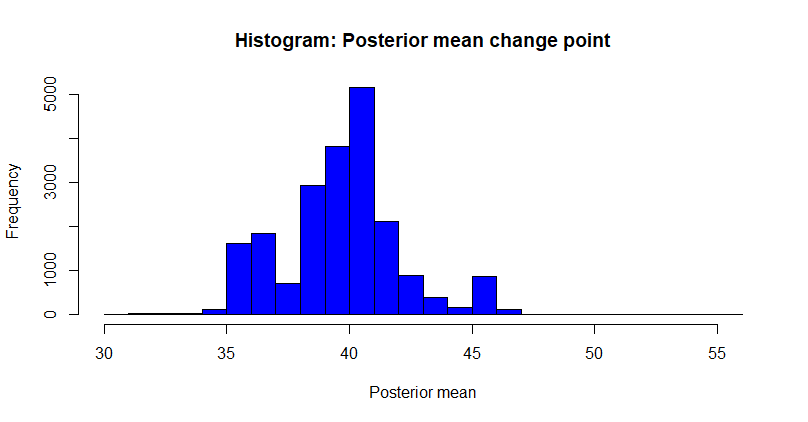
\includegraphics[width=340pt, height=200pt]{Chapters/chapter5/figures/Mining.png}
	%%\centerline{\epsfig{/Chapters/chapter1/figures/cat.eps,width=.8\textheight,height=.4\textwidth}}
	\caption[List of figure caption goes here]{Histogram of posterior draws of change point: Mining disasters}\label{fig52}
\end{figure} 

\subsection{Metropolis-Hastings}\label{sec512}

The Metropolis-Hastings (M-H) algorithm \cite{metropolis53,hastings70} is a general MCMC method that does not require standard closed-form solutions for the conditional posterior distributions. The key idea is to use a transition kernel whose unique invariant distribution is $\pi(\bm{\theta} | \bm{y})$. This kernel must satisfy the \textit{balancing condition}, meaning that, given a realization $\bm{\theta}^{(s-1)}$ at stage $s-1$ from the stationary distribution $\pi(\bm{\theta} | \bm{y})$, we generate a candidate draw $\bm{\theta}^{c}$ from the \textit{proposal distribution} $q(\bm{\theta}^{c} | \bm{\theta}^{(s-1)})$ at stage $s$ such that:
\[
q(\bm{\theta}^{c} | \bm{\theta}^{(s-1)}) \pi(\bm{\theta}^{(s-1)} | \bm{y}) = q(\bm{\theta}^{(s-1)} | \bm{\theta}^{c}) \pi(\bm{\theta}^{c} | \bm{y}),
\]

which implies that the probability of moving from $\bm{\theta}^{(s-1)}$ to $\bm{\theta}^{c}$ is equal to the probability of moving from $\bm{\theta}^{c}$ to $\bm{\theta}^{(s-1)}$.

In general, the \textit{balancing condition} is not automatically satisfied, and we must introduce an acceptance probability $\alpha(\bm{\theta}^{(s-1)}, \bm{\theta}^{c})$ to ensure that the condition holds:
\[
q(\bm{\theta}^{c} | \bm{\theta}^{(s-1)}) \pi(\bm{\theta}^{(s-1)} | \bm{y}) \alpha(\bm{\theta}^{(s-1)}, \bm{\theta}^{c}) = q(\bm{\theta}^{(s-1)} | \bm{\theta}^{c}) \pi(\bm{\theta}^{c} | \bm{y}).
\]

Thus, the acceptance probability is given by:

\[
\alpha(\bm{\theta}^{(s-1)}, \bm{\theta}^{c}) = 
\min\left\{\frac{q(\bm{\theta}^{(s-1)} | \bm{\theta}^{c}) \pi(\bm{\theta}^{c} | \bm{y})}{q(\bm{\theta}^{c} | \bm{\theta}^{(s-1)}) \pi(\bm{\theta}^{(s-1)} | \bm{y})}, 1\right\},
\]

where $q(\bm{\theta}^{c} | \bm{\theta}^{(s-1)})$ and $\pi(\bm{\theta}^{(s-1)} | \bm{y})$ must be nonzero, as transitioning from $\bm{\theta}^{(s-1)}$ to $\bm{\theta}^{c}$ is only possible under these conditions.

Algorithm \ref{Alg:MH} shows how to implement a Metropolis-Hastings algorithm. 

\begin{algorithm}[h!]
	\caption{Metropolis-Hastings algorithm}\label{Alg:MH}
	\begin{algorithmic}[1]
		\State Set $\bm{\theta}^{(0)}$ in the support of $\pi(\bm{\theta}|\bm{y})$  		 			
		\For{\texttt{$s=1,\dots,S$}}
		\State Draw $\bm{\theta}^{c}$ from $q(\bm{\theta}^{c}|\bm{\theta}^{(s-1)})$
		\State Calculate $\alpha(\bm{\theta}^{(s-1)}, \bm{\theta}^{c}) = 
		\min\left\{\frac{q(\bm{\theta}^{(s-1)} | \bm{\theta}^{c}) \pi(\bm{\theta}^{c} | \bm{y})}{q(\bm{\theta}^{c} | \bm{\theta}^{(s-1)}) \pi(\bm{\theta}^{(s-1)} | \bm{y})}, 1\right\}$
		\State Draw $U$ from $U(0,1)$
		\State $\bm{\theta}^{(s)}=\begin{Bmatrix}
			\bm{\theta}^{c} & \text{if } U\leq \alpha(\bm{\theta}^{(s-1)}, \bm{\theta}^{c})\\
			\bm{\theta}^{(s-1)} & \text{otherwise}\\
		\end{Bmatrix}$
		\EndFor 
	\end{algorithmic} 
\end{algorithm}

Some remarks: First, we do not need to know the marginal likelihood to implement the M-H algorithm, as it cancels out when calculating the acceptance probability. Second, the Gibbs sampling algorithm is a particular case of the M-H algorithm where the acceptance probability is equal to 1 (\cite{Gelman1992} and \cite[Chap.~10]{robert2011monte}, see Exercise 2). Third, we can combine the M-H and Gibbs sampling algorithms when dealing with relatively complex posterior distributions. Specifically, the Gibbs sampling algorithm can be used for blocks with conditional posterior distributions in standard closed forms, while the M-H algorithm is applied to sample from conditional posterior distributions that do not have standard forms. This approach is known as the M-H within Gibbs sampling algorithm. Fourth, we can note that the transition kernel in the M-H algorithm is a mixture of a continuous density ($q(\bm{\theta}^{c} | \bm{\theta}^{(s-1)})$) and a probability mass function ($\alpha(\bm{\theta}^{(s-1)}, \bm{\theta}^{c})$) \cite{chib1995understanding}. 

Fifth, a crucial point associated with the proposal densities is the acceptance probability. Low or high acceptance probabilities are not ideal. A low rate implies poor mixing, meaning the chain does not move effectively through the support of the posterior distribution. Conversely, a high acceptance rate implies that the chain will converge too slowly. A sensible value depends on the dimension of the parameter space. A rule of thumb is that if the dimension is less than or equal to 2, the acceptance rate should be around 0.50. If the dimension is greater than 2, the acceptance rate should be approximately 0.25 \cite{Roberts1997}. For technical details of the Metropolis-Hastings algorithm, see \cite[Chap.~7]{robert2011monte}.

Regarding the proposal density, it must be positive everywhere the posterior distribution is positive. This ensures that the Markov chain can explore the entire support of the posterior distribution. Additionally, the proposal density must allow the Markov chain to reach any region of the posterior distribution's support. There are three standard approaches for choosing the proposal density: the independent proposal, the random walk proposal, and the tailored proposal.

In the independent proposal, $q(\bm{\theta}^{c} | \bm{\theta}^{(s-1)}) = q(\bm{\theta}^{c})$, which implies that 

\[
\alpha(\bm{\theta}^{(s-1)}, \bm{\theta}^{c}) = 
\min\left\{\frac{q(\bm{\theta}^{(s-1)}) \pi(\bm{\theta}^{c} | \bm{y})}{q(\bm{\theta}^{c}) \pi(\bm{\theta}^{(s-1)} | \bm{y})}, 1\right\}.
\]

In this case, a move from $\bm{\theta}^{(s-1)}$ to $\bm{\theta}^{c}$ is always accepted if $q(\bm{\theta}^{(s-1)}) \pi(\bm{\theta}^{c} | \bm{y}) \geq q(\bm{\theta}^{c}) \pi(\bm{\theta}^{(s-1)} | \bm{y})$.

In the random walk proposal, $\bm{\theta}^{c} = \bm{\theta}^{(s-1)} + \bm{\epsilon}$, where $\bm{\epsilon}$ is a random perturbation. If $p(\bm{\epsilon}) = p(-\bm{\epsilon})$, meaning the distribution of $p(\bm{\epsilon})$ is symmetric around zero, then $q(\bm{\theta}^{c} | \bm{\theta}^{(s-1)}) = q(\bm{\theta}^{(s-1)} | \bm{\theta}^{c})$. Consequently, 

\[
\alpha(\bm{\theta}^{(s-1)}, \bm{\theta}^{c}) = 
\min\left\{\frac{\pi(\bm{\theta}^{c} | \bm{y})}{\pi(\bm{\theta}^{(s-1)} | \bm{y})}, 1\right\}.
\]

In this case, a move from $\bm{\theta}^{(s-1)}$ to $\bm{\theta}^{c}$ is always accepted if $\pi(\bm{\theta}^{c} | \bm{y}) \geq \pi(\bm{\theta}^{(s-1)} | \bm{y})$.

In the tailored proposal, the density is designed to have fat tails, is centered at the mode of the posterior distribution, and its scale matrix is given by the negative inverse Hessian matrix evaluated at the mode. Specifically, for two blocks, the log posterior distribution is maximized with respect to $\bm{\theta}_1$ given $\bm{\theta}_2$. This process is repeated at each iteration of the algorithm because $\bm{\theta}_2$ changes at different stages. As a result, the algorithm can be slow since the optimization process is computationally demanding (see \cite[Chap.~7 and 9]{greenberg2012introduction} for examples).

A sensible recommendation when performing M-H algorithm is to use a random walk proposal such that $\bm{\epsilon}\sim N(\bm{0},c^2\bm{\Sigma})$, where $\bm{\Sigma}$ is the negative inverse Hessian matrix evaluated at the mode, that is, maximize with respect to all parameters, and set $c\approx 2.4/\sqrt{dim\left\{\bm{\theta}\right\}}$, which is the most efficient scale compared to independent sampling \cite[Chap.~12]{gelman2021bayesian}. After some iterations of the algorithm, adjust the scale matrix $\bm{\Sigma}$ as before, and increase or decrease $c$ if the acceptance rate of the simulations is too high or low, respectively. The objective is to bring the acceptance rate to the stated rule of thumb, that is, if the dimension is less than or equal to 2, the acceptance rate should be around 0.50, and if the dimension is greater than 2, the acceptance rate should be around 0.25. Once this is achieved, we should run the algorithm without modifications and use this part of the algorithm to perform inference.\\


\textbf{Example: Ph.D. students sleeping hours continues}

In the Ph.D. students sleeping hours exercise of Chapter \ref{chap4} we get a posterior distribution that is Beta with parameters 16.55 and 39.57. We can sample from this posterior distribution using the function \textit{rbeta} from \textbf{R}. However, we want to compare the performance of a M-H algorithm using as proposal density a $U(0,1)$ distribution.

The following code shows how to do a M-H algorithm to sample from the beta distribution using the uniform distribution.

\begin{tcolorbox}[enhanced,width=4.67in,center upper,
	fontupper=\large\bfseries,drop shadow southwest,sharp corners]
	\textit{R code. Metropolis-Hastings algorithm:  Ph.D. students sleeping hours}
	\begin{VF}
		\begin{lstlisting}[language=R]
rm(list = ls()); set.seed(010101)
an <- 16.55; bn <- 39.57
S <- 100000; p <- runif(S); acept <- rep(0, S)
for (s in 2:S){
	pc <- runif(1) # Candidate
	a <- dbeta(pc, an, bn)/dbeta(p[s-1], an, bn) # Acceptance rate
	U <- runif(1)
	if(U <= a){
		p[s] <- pc
		acept[s] <- 1
	}else{
		p[s] <- p[s-1]
		acept[s] <- 0
	}
}
mean(acept); mean(p); sd(p)
an/(an + bn); (an*bn/((an+bn)^2*(an+bn+1)))^0.5 # Population values
h <- hist(p, breaks=50, col="blue", xlab="Proportion Ph.D. students sleeping at least 6 hours", main="Beta draws from a Metropolis-Hastings algorithm")
pfit <- seq(min(p),max(p),length=50)
yfit<-dbeta(pfit, an, bn)
yfit <- yfit*diff(h$mids[1:2])*length(p)
lines(pfit, yfit, col="red", lwd=2)
\end{lstlisting}
	\end{VF}
\end{tcolorbox} 

The results indicate that the mean and standard deviation obtained from the posterior draws are similar to the population values. Furthermore, Figure \ref{fig53} presents the histogram of the posterior draws alongside the density of the beta distribution, demonstrating a good match between them.

\begin{figure}[!h]
	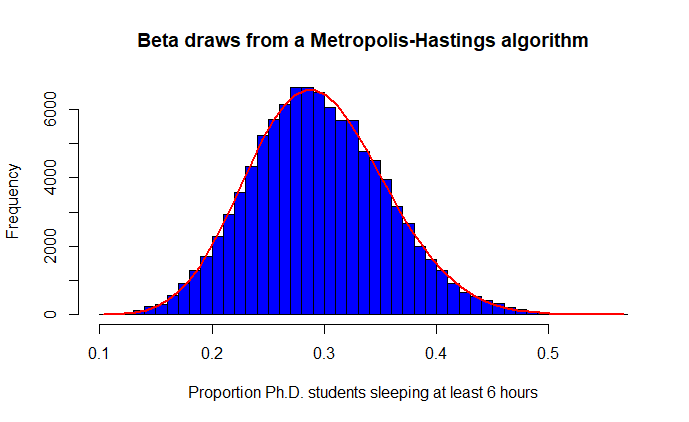
\includegraphics[width=340pt, height=200pt]{Chapters/chapter5/figures/Beta.png}
	%%\centerline{\epsfig{/Chapters/chapter1/figures/cat.eps,width=.8\textheight,height=.4\textwidth}}
	\caption[List of figure caption goes here]{Histogram of posterior draws of beta distribution and the density of the beta distribution.}\label{fig53}
\end{figure}      

\subsection{Hamiltonian Monte Carlo}\label{sec523}

Hamiltonian Monte Carlo (HMC) is an extension of the Metropolis algorithm designed to efficiently explore the parameter space by introducing \textit{momentum variables}. It is particularly advantageous for high-dimensional posterior distributions, as it reduces the risk of getting stuck in local modes and significantly improves mixing. HMC leverages concepts from physics, specifically Hamiltonian mechanics, to propose transitions in the Markov chain.

\section{Importance sampling}\label{sec52}

\section{Sequential Monte Carlo}\label{sec53}

\section{Convergence diagnostics}\label{sec54}
\subsection{Numerical standard error}
\subsection{Effective sample size}
\subsection{Checking for errors in the posterior simulator}
\cite{geweke2004getting}

\section{Summary}\label{sec55}


\section{Exercises}\label{sec56}

\begin{enumerate}
	\item \textbf{Example: The normal model with independent priors}
	
	Let's recap the math test exercise in Chapter \ref{chap4}, this time assuming independent priors. Specifically, let $Y_i \sim N(\mu, \sigma^2)$, where $\mu \sim N(\mu_0, \sigma_0^2)$ and $\sigma^2 \sim IG(\alpha_0 / 2, \delta_0 / 2)$. The sample size is 50, and the mean and standard deviation of the math scores are 102 and 10, respectively. We set $\mu_0 = 100$, $\sigma_0^2 = 100$, and $\alpha_0 = \delta_0 = 0.001$.
	
	\begin{itemize}
		\item Find the posterior distribution of $\mu$ and $\sigma^2$.
		\item Program a Gibbs sampler algorithm and plot the histogram of the posterior draws of $\mu$
	\end{itemize}

	\item Show that the Gibbs sampler is a particular case of the Metropolis-Hastings where the acceptance probability is equal to 1.
	
	\item Implement a Metropolis-Hastings to sample from the Cauchy distribution, $C(0,1)$, using as proposal a standard normal distribution and a Student's t distribution with 5 degree of freedom.  
	
\end{enumerate}



